% A LaTeX (non-official) template for ISAE projects reports
% Copyright (C) 2014 Damien Roque
% Version: 0.2
% Author: Damien Roque <damien.roque_AT_isae.fr>

\documentclass[a4paper,12pt]{book}
\usepackage[utf8]{inputenc}
\usepackage[T1]{fontenc}
\usepackage[english]{babel} % If you write in English
\usepackage{a4wide}
\usepackage{graphicx}
\graphicspath{{images/}}
\usepackage{subfig}
\usepackage{tikz}
\usetikzlibrary{shapes,arrows}
\usepackage{pgfplots}
\pgfplotsset{compat=newest}
\pgfplotsset{plot coordinates/math parser=false}
\newlength\figureheight
\newlength\figurewidth
\pgfkeys{/pgf/number format/.cd,
set decimal separator={,\!},
1000 sep={\,},
}
\usepackage{ifthen}
\usepackage{ifpdf}
\usepackage{enumitem}
\ifpdf
\usepackage[pdftex]{hyperref}
\else
\usepackage{hyperref}
\fi
\usepackage{color}
\hypersetup{%
colorlinks=true,
linkcolor=black,
citecolor=black,
urlcolor=black}

\renewcommand{\baselinestretch}{1.05}
\usepackage{fancyhdr}
\pagestyle{fancy}
\fancyfoot{}
\fancyhead[LE,RO]{\bfseries\thepage}
\fancyhead[RE]{\bfseries\nouppercase{\leftmark}}
\fancyhead[LO]{\bfseries\nouppercase{\rightmark}}
\setlength{\headheight}{15pt}

\let\headruleORIG\headrule
\renewcommand{\headrule}{\color{black} \headruleORIG}
\renewcommand{\headrulewidth}{1.0pt}
\usepackage{colortbl}
\arrayrulecolor{black}

\fancypagestyle{plain}{
  \fancyhead{}
  \fancyfoot[C]{\thepage}
  \renewcommand{\headrulewidth}{0pt}
}

\makeatletter
\def\@textbottom{\vskip \z@ \@plus 1pt}
\let\@texttop\relax
\makeatother

\makeatletter
\def\cleardoublepage{\clearpage\if@twoside \ifodd\c@page\else%
  \hbox{}%
  \thispagestyle{empty}%
  \newpage%
  \if@twocolumn\hbox{}\newpage\fi\fi\fi}
\makeatother

\usepackage{amsthm}
\usepackage{amssymb,amsmath,bbm}
\usepackage{array}
\usepackage{bm}
\usepackage{multirow}
\usepackage[footnote]{acronym}

\newcommand*{\SET}[1]  {\ensuremath{\mathbf{#1}}}
\newcommand*{\VEC}[1]  {\ensuremath{\boldsymbol{#1}}}
\newcommand*{\FAM}[1]  {\ensuremath{\boldsymbol{#1}}}
\newcommand*{\MAT}[1]  {\ensuremath{\boldsymbol{#1}}}
\newcommand*{\OP}[1]  {\ensuremath{\mathrm{#1}}}
\newcommand*{\NORM}[1]  {\ensuremath{\left\|#1\right\|}}
\newcommand*{\DPR}[2]  {\ensuremath{\left \langle #1,#2 \right \rangle}}
\newcommand*{\calbf}[1]  {\ensuremath{\boldsymbol{\mathcal{#1}}}}
\newcommand*{\shift}[1]  {\ensuremath{\boldsymbol{#1}}}

\newcommand{\eqdef}{\stackrel{\mathrm{def}}{=}}
\newcommand{\argmax}{\operatornamewithlimits{argmax}}
\newcommand{\argmin}{\operatornamewithlimits{argmin}}
\newcommand{\ud}{\, \mathrm{d}}
\newcommand{\vect}{\text{Vect}}
\newcommand{\sinc}{\ensuremath{\mathrm{sinc}}}
\newcommand{\esp}{\ensuremath{\mathbb{E}}}
\newcommand{\hilbert}{\ensuremath{\mathcal{H}}}
\newcommand{\fourier}{\ensuremath{\mathcal{F}}}
\newcommand{\sgn}{\text{sgn}}
\newcommand{\intTT}{\int_{-T}^{T}}
\newcommand{\intT}{\int_{-\frac{T}{2}}^{\frac{T}{2}}}
\newcommand{\intinf}{\int_{-\infty}^{+\infty}}
\newcommand{\Sh}{\ensuremath{\boldsymbol{S}}}
\newcommand{\C}{\SET{C}}
\newcommand{\R}{\SET{R}}
\newcommand{\Z}{\SET{Z}}
\newcommand{\N}{\SET{N}}
\newcommand{\K}{\SET{K}}
\newcommand{\reel}{\mathcal{R}}
\newcommand{\imag}{\mathcal{I}}
\newcommand{\cmnr}{c_{m,n}^\reel}
\newcommand{\cmni}{c_{m,n}^\imag}
\newcommand{\cnr}{c_{n}^\reel}
\newcommand{\cni}{c_{n}^\imag}
\newcommand{\tproto}{g}
\newcommand{\rproto}{\check{g}}
\newcommand{\LR}{\mathcal{L}_2(\SET{R})}
\newcommand{\LZ}{\ell_2(\SET{Z})}
\newcommand{\LZI}[1]{\ell_2(\SET{#1})}
\newcommand{\LZZ}{\ell_2(\SET{Z}^2)}
\newcommand{\diag}{\operatorname{diag}}
\newcommand{\noise}{z}
\newcommand{\Noise}{Z}
\newcommand{\filtnoise}{\zeta}
\newcommand{\tp}{g}
\newcommand{\rp}{\check{g}}
\newcommand{\TP}{G}
\newcommand{\RP}{\check{G}}
\newcommand{\dmin}{d_{\mathrm{min}}}
\newcommand{\Dmin}{D_{\mathrm{min}}}
\newcommand{\Image}{\ensuremath{\text{Im}}}
\newcommand{\Span}{\ensuremath{\text{Span}}}

\newtheoremstyle{break}
  {11pt}{11pt}%
  {\itshape}{}%
  {\bfseries}{}%
  {\newline}{}%
\theoremstyle{break}

%\theoremstyle{definition}
\newtheorem{definition}{Définition}[chapter]

%\theoremstyle{definition}
\newtheorem{theoreme}{Théorème}[chapter]

%\theoremstyle{remark}
\newtheorem{remarque}{Remarque}[chapter]

%\theoremstyle{plain}
\newtheorem{propriete}{Propriété}[chapter]
\newtheorem{exemple}{Exemple}[chapter]

\parskip=5pt
%\sloppy

\begin{document}

%%%%%%%%%%%%%%%%%%
%%% First page %%%
%%%%%%%%%%%%%%%%%%

\begin{titlepage}
\begin{center}

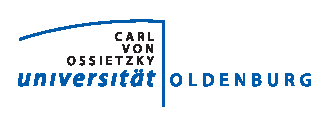
\includegraphics[width=0.6\textwidth]{uol}\\[1cm]

{\large Modellierungspraktikum}\\[0.5cm]

{\large SS 2019}\\[0.5cm]

% Title
\rule{\linewidth}{0.5mm} \\[0.4cm]
{ \huge \bfseries Cross Correlation of two Ohrnstein Uhlenbeck Processes with Delayed Noise \\[0.4cm] }
\rule{\linewidth}{0.5mm} \\[1.5cm]

% Author and supervisor
\noindent
\begin{minipage}{0.4\textwidth}
  \begin{flushleft} \large
    \emph{Author}\\
    Tjark Smalla\\
  \end{flushleft}
\end{minipage}%
\begin{minipage}{0.4\textwidth}
  \begin{flushright} \large
    \emph{Professor} \\
    PD. Jan Freund
  \end{flushright}
\end{minipage}

\vfill

% Bottom of the page
{\large \today}

\end{center}
\end{titlepage}

%%%%%%%%%%%%%%%%%%%%%%%%%%%%%
%%% Non-significant pages %%%
%%%%%%%%%%%%%%%%%%%%%%%%%%%%%

\frontmatter

\tableofcontents

\clearpage
\listoffigures

\clearpage
\chapter*{Acronyms}
\begin{acronym}[CP-OFDMX] % Give the longest acronym here
\acro{OU}{Ohrnstein Uhlenbeck}
\acro{CCF}{cross correlation function}
\acro{ACF}{auto correlation function}
\acro{SDE}{stochastic differential equation}
\acro{EM}{Euler-Maruyama Method}
\acro{FWAHH}{Full Width at Half Height}
\end{acronym}

%%%%%%%%%%%%%%%%%%%%%%%%%%%%%%%%%%%%%%%%%%%%
%%% Content of the report and references %%%
%%%%%%%%%%%%%%%%%%%%%%%%%%%%%%%%%%%%%%%%%%%%

\mainmatter
\pagestyle{fancy}

\cleardoublepage
\chapter{Introduction}\label{ch/intro}
Aim of this report is to study the \ac{CCF} properties of two connected \ac{OU} processes under changing parameterization.
Both processes are powered by gaussian noise, whereas the second process is powered by a linear combination of a time delayed version of the first noise and a second gaussian noise process. The two independent gaussian noise processes will be from now on referred to as noise 1 and noise 2. The noise resulting from the linear combination of noise 1 and noise 2 will be referred to as mixed noise. Noise 1 is powering \ac{OU} process 1 and the mixed noise powers \ac{OU} process 2. For better readability, the first process is from now on referred to as OU1 and the second process as OU2.
To further analyze the dependency of the \ac{CCF}s characteristics on the noise, the gaussian noise is replaced by a red noise.
The current chapter is supposed to define the model under study(\ref{s/model})) as well as which parameters will be analyzed(\ref{s/intro/parameter}).
Chapter \ref{ch/methodology} explains how the effects on the \ac{CCF} by different parameterization where researched. Section \ref{s/meth/num} explains in more detail which method was used to solve the \ac{SDE} defined in equation \ref{m/ou1n} and \ref{m/ou2n} while section \ref{s/meth/simulation} gives an overview over the simulation parameters and methods.

\section{Model Definition}\label{s/model}
The \ac{OU} processes under study are given by following langevin equations

\begin{equation}\label{m/ou1}
	\dot{x_1}=-\frac{x_1}{\tau_1} + \sqrt{\frac{2\sigma^2}{\tau_1}}\xi_1(t)
\end{equation}

\begin{equation}\label{m/ou2}
	\dot{x_2}=-\frac{x_2}{\tau_2} + \sqrt{\frac{2\sigma^2}{\tau_2}}\times[\sqrt{\epsilon^2}\xi_1(t - T) + \sqrt{1-\epsilon^2} \xi_2(t)]
\end{equation}
with relaxation rate $\tau$, noise intensity $\sigma^2$ and coupling delay $T$.
Assuming a shared dimension of $x_1$ and $x_2$, the $\sigma$ can assumed to be 1 which leads to following normalized processes:

\begin{equation}\label{m/ou1n}
\dot{x_1}=-\frac{x_1}{\tau_1} + \sqrt{\frac{2}{\tau_1}}\xi_1(t)
\end{equation}

\begin{equation}\label{m/ou2n}
\dot{x_2}=-\frac{x_2}{\tau_2} + \sqrt{\frac{2}{\tau_2}}\times[\sqrt{\epsilon^2}\xi_1(t - 1) + \sqrt{1-\epsilon^2} \xi_2(t)].
\end{equation}

The impact of the noises \ac{ACF} properties is studied by assuming white and red spectral characteristics. Thus the \ac{ACF} of noise 1 and 2($\xi_1$, $\xi_2$) is given by

% TODO add comment for cases red and white nosie behin the condition
% TODO remake sentence before equation
\begin{equation}
	\langle x_i(t)x_j(s)\rangle = \delta_{i,j}
	\begin{cases} 
	\delta(t-s) \\
	e^{-\gamma_i |t-s|}
	\end{cases}
\end{equation}

with $\gamma$ controlling the correlation time of the the red noise.

\section{Parameter Under Study}\label{s/intro/parameter}
Special attention is given to the effects resulting from changes in the parameters controlling the weighting of the linear combination ($\epsilon$), the relaxation intensity controlling $\tau$ as well $\gamma$ which controls the correlation time of the red noise.

% TODO Expectation

% --------------------------------------------------------------------------------------------
\chapter{Methodology}\label{ch/methodology}
To analyze parameterization effects on the \ac{ACF}s and \ac{CCF}s, both are estimated from an ensemble of bivariate time series generated from the \ac{SDE} defined in equation \ref{m/ou1n} and \ref{m/ou2n}. 
Simulation takes place in the time interval $[0, T_{cycles }* T]$.
Resulting \acf{ACF}s are analyzed for their correlation with a lag of a fifth of the total simulation time. 
\ac{CCF}s are analyzed with a lag in the interval $[T - \frac{T_{Total}}{10}, T + \frac{T_{Total}}{10}]$.
For the lags to be resolution independent, lags are calculated by $lag_t=\frac{t*R}{T_Total}$.
Following parameters control the simulation:

\begin{itemize}
	\item T - The time delay of noise 1 inside the mixed noise. Always 1.
	\item R - Resolution of the simulated time range.
	\item ensembles - Number of simulation runs used for estimation
	\item T\textunderscore cycles - Determines the time range for the simulation. The simulation is done in the range of $t\in[0, T*T\textunderscore cycles]  $. Always 2.
	\item Initial\textunderscore Condition - Initial condition for both \ac{OU} processes. The initial condition was chosen to be always zero for easier visualization of the \ac{CCF} results.
	\item $\epsilon$ - Weighting for the linear combination of noise 1 and noise 2 in mixed noise. $\epsilon_i \in [0, 1]$.
	\item $\tau_i$ - Relaxation coefficient of the i-th \ac{OU} process
	\item Noise Type - Determines spectral properties of noise 1 and 2, which is either red or white.
	\item $\gamma_i$ - Correlation coefficient of the i-th red noise. $\gamma_i \in [0, 1]$.
\end{itemize}.

Three different parameter sets where chosen to study different research questions. The first set is used to find differences in the \ac{ACF}/\ac{CCF} behavior caused by different spectral properties of the OU powering noise processes. Also it is used to find effects of symmetrical changes to $\tau_1$/$\tau_2$ and $\epsilon$. The second set is used to study effects of asymmetric changes to $\tau_1$/$\tau_2$ whereas the third set focuses on asymmetric changes to $\gamma_1$/$\gamma_2$.
Details for each parameters set can be taken from table \ref{t/a/parameterSet1}, \ref{t/a/parameterSet2} and \ref{t/a/parameterSet3} in chapter \ref{ch/appendix}.

\section{Software}
The simulation was written in the python programming language. Freely available packages were used to simplify simulation and result analysis. A complete list of used packages and their versions can be found in the file \emph{requirements.txt}. The source code can be found under \hyperlink{https://github.com/ChillkroeteTTS/ccf-analysis-of-two-coupled-ou-processes}{https://github.com/ChillkroeteTTS/ccf-analysis-of-two-coupled-ou-processes}.
Simulations where started from the file \emph{src/main\_multiple\_runs.py}, analysis took place in Jupyter Notebooks which are located under \emph{src/notebooks}. Notebook \emph{src/notebooks/noise\_validation.ipynb} was used to validate that the simulated noise intensity of noise 1 and mixed noise was always 1.

\section{Numerical Integration}\label{s/meth/num}
To estimate a numerical solution to the \ac{SDE}s defined in chapter \ref{ch/intro}, the \ac{EM} was used.
As described in \cite{numSim}, in order to solve a \ac{SDE}

\begin{equation}\label{eq/meth/num/sde}
	dX(t) = f(X(t)dt) + g(X(t))dW(t), X(0)=X_0, 0 \le t \le T
\end{equation} numerically, it has to be discretized.
Note that $f(X(t))$ is the drift term, $G(X(t))$ is the diffusion term and $dW(t)$ the  Wiener increment.

Let $\Delta t$ be $T_{Total}/R$ and $t_i = i\Delta t$, the \ac{SDE} from section \ref{s/model} looks as following in the \ac{EM} form:


\begin{equation}\label{eq/meth/num/discSde}
	x_i = x_{i-1} -\frac{x_i}{\tau_i} \Delta t + \sqrt{\frac{2}{\tau_i}} (W(t_i)  - W(t_{i-1})), i=1,2,..., T_{Total}
\end{equation}.

With $\Delta W = W(t_i)  - W(t_{i-1})$ being independent and normally distributed with mean zero and variance $t_i - t_{i-1} = \Delta t$. Thus, it can be assumed that $\Delta W \sim N(0, \Delta t)$ where $N(0, \Delta t)$ denotes a normal distributed random variable with a mean  of zero and a variance of $\Delta t$. 

\section{Behavior of Mixed Noise for t < T}\label{s/meth/simulation}
OU1 is powered by  and OU2 by the mixed noise which is a combination of noise 2 and a by $T$ delayed version of noise 1.
However, the noise1 process is only defined for the interval $[0, T_{cycles} * T]$ which lefts the mixed noise process undefined for $t < T$ since $t - T$ is negative. 
Thus, $mixed\_noise(t) = noise2(t)  \quad \forall t < T$ was defined.



% --------------------------------------------------------------------------------------------
\chapter{Results}\label{ch/results}
A total of X parameter sets with an ensemble of Y simulation runs were performed in order to estimate the ACFs and CCFs of the processes defined in section \ref{s/model}. Section \ref{s/r/overview} provides an overview about the generated functions for parameter sets with a symmetry condition of $\tau_1 = \tau_2$ and $\gamma_1 = \gamma_2$. dection C presents correlations between parameterization and key features of the discussed functions. Finally, section shows effects which become apparent for parameter sets where the pairs of $\tau$ and $\gamma$ are not equal anymore.

The median, the 25\% and the 75\% percentile are build across each ACF/CCF for each simulation run. The resulting median functions are used for comparison between parameter sets.

\section{Estimated ACFs and CCFs of Simulated Processes}\label{s/r/overview}
It is expected to see a high auto correlation for processes with a high relaxation coefficient $\tau$. Although figure \ref{f/r/acf_white_sym} shows a minimal increase of such a behavior in the estimated ACFs, a clear correlation can not be seen clearly.
Looking at the CCFs in figure \ref{f/r/ccf_white_sym} on the other hand shows clearly an increasingly high peak  with rising $\epsilon$ which was expected.
To compare the range of time offsets in which both processes are correlated, the \ac{FWAHH} was calculated and displayed. However, a clear increase or decrease in the FWAHH can not be seen in figure \ref{f/r/ccf_white_sym}.

Since processes powered by red noise showed the same behavior as the ones powered by white noise, their ACF and CCF estimations can be found in the appendix in figure \ref{f/a/acf_red_sym} and \ref{f/a/ccf_red_sym}.

\begin{figure}[htp]
	\includegraphics[width=1.\textwidth]{../results/params_symmetric_increasing_taus_300_700_0/.images/white_noise_acf}%
	\caption{Median of the estimated ACFs for parameter sets with white noise and symmetry condition. Sets with increasing $\epsilon$ are displayed from left to right, sets with increasing $\tau$ from top to bottom. The area resembles the 25\% and 75\% percentile. The height of the function at a lag of 0.08 is marked for comparison. Note the slight correlation rise with increasing $\tau$ }%
	\label{f/r/acf_white_sym}%
\end{figure}

\begin{figure}[htp]
	\includegraphics[width=1.\textwidth]{../results/params_symmetric_increasing_taus_300_700_0/.images/white_noise_ccf}%
	\caption{Median of the estimated CCFs for parameter sets with white noise and symmetry condition. Sets with increasing $\epsilon$ are displayed from left to right, sets with increasing $\tau$ from top to bottom. The area resembles the 25\% and 75\% percentile. The \ac{FWAHH} of the function is marked for comparison. Note the rise of the peak height with increasing $\epsilon$. }%
	\label{f/r/ccf_white_sym}
\end{figure}


\section{Correlation between ACF/CCF Behavior and Parameterization}\label{s/r/correlation_sym}
As already seen in section \ref{s/r/overview}, the ACFs show a stronger auto correlation with rising $\tau$ and a higher cross correlation with rising $\epsilon$. This behavior is confirmed by figure \ref{f/r/acf_white_sym_correlation} and \ref{f/r/ccf_white_sym_correlation_height}, which show that only only one of both parameters lead to an increase in their respective property.
However, it is interesting to see, that the correlation between $\tau$ and the auto correlation does not appear linear.
An interesting property of the CCF is shown in Figure \ref{f/r/ccf_white_sym_correlation_width}. The width of the CCF seems to correlate with the relaxation parameter $\tau$.
Since the ACFs of both OU processes exhibit the same behavior, only the contour plot for OU1 is shown. The corresponding plot for OU2 can be found in figure \ref{f/a/acf_white_sym_correlation_ou2}.
As in section \ref{s/r/overview} suggested, no difference between white and red  noise powered processes  can be seen.

\begin{figure}[htp]
	\includegraphics[width=1.\textwidth]{../results/params_symmetric_increasing_taus_300_700_0/.images/acf_correlation_ou1}%
	\caption{Contour plot showing the correlation between $\tau$, $\epsilon$ and the auto correlation at a lag of 0.08 for white (left ) and red(right) noise powered processes. Note how the correlation rise is not linear. The datapoints  the contour plot is based on are shown by the blue crosses.}%
	\label{f/r/acf_white_sym_correlation}%
\end{figure}

\begin{figure}[htp]
	\includegraphics[width=1.\textwidth]{../results/params_symmetric_increasing_taus_300_700_0/.images/ccf_peak_height_correllation}%
	\caption{Contour plot showing the correlation between $\tau$, $\epsilon$ and the peak height of the CCF median for white (left ) and red(right) noise. A clear, linear dependents of the maximum peak height on $\epsilon$ can be seen. The datapoints  the contour plot is based on are shown by the blue crosses.}%
	\label{f/r/ccf_white_sym_correlation_height}
\end{figure}

\begin{figure}[htp]
	\includegraphics[width=1.\textwidth]{../results/params_symmetric_increasing_taus_300_700_0/.images/ccf_fwahh_correlation}%
	\caption{Contour plot showing the correlation between $\tau$, $\epsilon$ and the \ac{FWAHH} of the CCF median for white (left ) and red(right) noise. A clear, linear correlation of the width on $\tau$ can be seen. The datapoints  the contour plot is based on are shown by the blue crosses. }%
	\label{f/r/ccf_white_sym_correlation_width}
\end{figure}

\subsection{Asymmetric $\tau_1$ and $\tau_2$}
Paramet 


% --------------------------------------------------------------------------------------------
\chapter{Conclusions}\label{ch/conclusion}
% TODO Mention further research on non linear rise of the auto correlation with tau

\chapter{Appendix}\label{ch/appendix}


\begin{table}\label{t/a/parameterSet1}
\begin{tabular}{ l | c | r }
		1 & 2 & 3 \\
		4 & 5 & 6 \\
		7 & 8 & 9 \\
		\hline  
	\end{tabular}
	\caption{\label{tab:table-name} Parameter Set 1}
\end{table}

\begin{table}\label{t/a/parameterSet2}
	\begin{tabular}{ l | c | r }
		1 & 2 & 3 \\
		4 & 5 & 6 \\
		7 & 8 & 9 \\
		\hline  
	\end{tabular}
	\caption{\label{tab:table-name} Parameter Set 2}
\end{table}

\begin{table}\label{t/a/parameterSet3}
	\begin{tabular}{ l | c | r }
		1 & 2 & 3 \\
		4 & 5 & 6 \\
		7 & 8 & 9 \\
		\hline  
	\end{tabular}
	\caption{\label{tab:table-name} Parameter Set 1}
\end{table}

\begin{figure}[htp]
	\includegraphics[width=1.\textwidth]{../results/params_symmetric_increasing_taus_300_700_0/.images/red_noise_acf}%
	\caption{Median of the estimated ACFs for parameter sets with red noise and symmetry condition. Sets with increasing $\epsilon$ are displayed from left to right, sets with increasing $\tau$ from top to bottom. The area resembles the 25\% and 75\% percentile. The height of the function at a lag of 0.08 is marked for comparison. Note the slight correlation rise with increasing $\tau$ }%
	\label{f/a/acf_red_sym}%
\end{figure}

\begin{figure}[htp]
	\includegraphics[width=1.\textwidth]{../results/params_symmetric_increasing_taus_300_700_0/.images/red_noise_ccf}%
	\caption{Median of the estimated CCFs for parameter sets with red noise and symmetry condition. Sets with increasing $\epsilon$ are displayed from left to right, sets with increasing $\tau$ from top to bottom. The area resembles the 25\% and 75\% percentile. The \ac{FWAHH} of the function is marked for comparison. Note the rise of the peak height with increasing $\epsilon$. }%
	\label{f/a/ccf_red_sym}
\end{figure}

\begin{figure}[htp]
	\includegraphics[width=1.\textwidth]{../results/params_symmetric_increasing_taus_300_700_0/.images/acf_correlation_ou2}%
	\caption{Contour plot showing the correlation between $\tau$, $\epsilon$ and the auto correlation at a lag of 0.08 for white (left ) and red(right) noise powered processes. Note how the correlation rise is not linear.}%
	\label{f/a/acf_white_sym_correlation_ou2}%
\end{figure}

\appendix

\bibliographystyle{plain}
\bibliography{references}

\clearpage

%%%%%%%%%%%%%%%%
%%% Abstract %%%
%%%%%%%%%%%%%%%%

\thispagestyle{empty}

\end{document}